%!TEX root = ../thesis.tex

\chapter{BEM with inexact GMRES for the Laplace equation}
\label{chapter:laplace_bem}
\thispagestyle{myheadings}

% set this to the location of the figures for this chapter. it may
% also want to be ../Figures/2_Body/ or something. make sure that
% it has a trailing directory separator (i.e., '/')!
\graphicspath{{Laplace/}}

To properly evaluate the utility of our relaxed {\fmm}-{\bem} method, we must apply it to a variety of examples, both to test for correctness (obtaining the correct answer and maintaining all convergence properties) and to evaluate the ``real-world'' potential for speedup.

% \section{Equation}\label{laplace:equation}

The first such example we will look at is the solution to Laplace's equation, consisting of obtaining $\phi(\vect{x})$ such that:

\begin{equation}\label{eqn:laplace}
	\nabla^{2}\phi(\vect{x}) = 0
\end{equation}

This equation can be used to model several applications, including electrostatics \cite{YokotaETal2010}, potential flow \cite{klaseboeretal2011} and heat transfer \cite{panti2008,majchrzakfreus2003}, and using {\fmmbem} in particular \cite{Nabors94}.

%By using the fundamental solution to \ref{eqn:laplace} we can write the potential at a point $\vect{x}_i$ from point $\vect{x}_j$ as a function of the distance between the two points,
%
%\begin{equation}\label{eqn:fundamental_laplace}
%	\phi(\vect{x}_i) = \frac{q_j}{|\vect{x}_i - \vect{x}_j|}.
%\end{equation}
%
%From the potential of a single pair of points, it is easy to find the influence from all points $\vect{x}_j,\; j=1..N$ at $\vect{x}_i$, as a simple $N$-body sum over \ref{eqn:fundamental_laplace}
%
%\begin{equation}
%	\phi(\vect{x}_i) = \sum_{j}^{N}\frac{q_j}{|\vect{x}_i - \vect{x}_j|}.
%\end{equation}
%
%These fundamental solutions, or Greens functions will be used later as part of the {\bem} formulation.

\section{BEM}\label{sec:bem_derivation}

To obtain a {\bem} formulation for Laplace, we start with the weak formulation of \ref{eqn:laplace}, with some weighting function, $W$,

\begin{equation}
	\int_{\Omega} \left [\nabla^{2}\phi\;W\right]\;\di{\Omega} = 0.
\end{equation}

We can write this in a different form,

\begin{equation}\label{eqn:laplace_weak_form}
	\int_{\Omega} \left [ \nabla(\nabla\phi\;W) - \nabla\phi\nabla W\right ] \;\di{\Omega} = 0.
\end{equation}

Applying Gauss' divergence theorem to the first term, we convert it into a surface integral, while simultaneous re-writing the second term, $\nabla\phi\nabla W = \nabla(\phi\nabla W) - \phi\nabla^{2}W$ gives us

\begin{equation}\label{eqn:laplace_bem_1}
	\int_{\Gamma}\left [ \nabla\phi\;W\cdot\nhat\right ]\;\di{\Gamma} - \int_{\Omega} \left [\nabla(\phi\nabla W) - \phi\nabla^{2}W\right ]\;\di{\Omega} = 0.
\end{equation}

Utilizing Gauss' divergence theorem once again, and choosing $W = G = 1/4\pi r$, the Green's function for the Laplace equation (while noting that $\nabla^{2}G = -\delta$), we obtain

\begin{equation}\label{eqn:laplace_bem_2}
	\int_{\Gamma}\partiald{\phi}{\nhat}G\;\di{\Gamma} - \int_{\Gamma} \phi\partiald{G}{\nhat}\;\di{\Gamma} - \int_{\Omega} \phi\nabla^{2}G\;\di{\Omega} = 0.
\end{equation}

Taking advantage of $\nabla^{2}G = -\delta$, we obtain the near-final form

\begin{equation}\label{eqn:laplace_bem_3}
	\int_{\Gamma}\partiald{\phi}{\nhat}G\;\di{\Gamma} - \int_{\Gamma} \phi\partiald{G}{\nhat}\;\di{\Gamma} - \phi = 0.
\end{equation}.

The final step we must perform is to take our target point, $i$, to the boundary, where we want to form a linear system. At $i$ we augment the domain by a small hemisphere around the point with radius $\epsilon$. We can then consider $i$ as $\epsilon \to 0$. The first integral to be treated is over $G$ as it presents a lower order singularity than the integral over $\partialdi{G}{\nhat}$.

\begin{eqnarray}
	\lim_{\epsilon\to0} \int_{\Gamma_\epsilon} G\partiald{\phi}{\nhat}\;\di{\Gamma} & = & \lim_{\epsilon\to0}\int_{\Gamma_\epsilon} \frac{1}{4\pi\epsilon}\partiald{\phi}{\nhat}\;\di{\Gamma} \\
	& = & \lim_{\epsilon\to0}\frac{2\epsilon^{2}}{4\pi\epsilon} \partiald{\phi}{\nhat} = 0
\end{eqnarray}

In a similar fashion, we take the integral over $\partialdi{G}{\nhat}$ to the surface,

\begin{eqnarray}
	\lim_{\epsilon\to0} \int_{\Gamma_\epsilon} \phi\partiald{G}{\nhat}\;\di{\Gamma} & = & -\lim_{\epsilon\to0} \int_{\Gamma_\epsilon} \phi\frac{1}{4\pi\epsilon^{2}} \\
	& = & -\lim_{\epsilon\to0} \phi\frac{2\pi\epsilon^{2}}{4\pi\epsilon^{2}} = -\frac{1}{2}\phi.
\end{eqnarray}

Utilizing these two results and applying them to equation \ref{eqn:laplace_bem_3} with some re-arrangement, we obtain the final form for the Laplace equation:

\begin{equation}\label{eqn:laplace_bem_final}
	\frac{1}{2}\phi + \int_{\Gamma} \phi\partiald{G}{\nhat}\;\di{\Gamma} = \int_{\Gamma}\partiald{\phi}{\nhat}G\;\di{\Gamma}.
\end{equation}

The constant of $1/2$ holds as long as target points are located on a smooth surface, that is to say, not on the edge or corner of a panel. As noted in \S\ref{sec:bem}, we use constant, flat panels with collocation, resulting in targets in the center of panels, allowing us to use this formulation with no changes.

%For a boundary element formulation for Laplace, we actually start from Poisson's equation, which will allow us to introduce any kind of additional sources, such as point charges, while setting $\vect{f} = 0$ recovers the standard Laplace's equation.
%
%\begin{equation}
%	\nabla^{2}\phi(\vect{x}) + \vect{f} = 0,
%	\label{eqn:poisson}
%\end{equation}
%
%\noindent
%Here $\vect{f} \in \R^{3}$ is a known function at all points. Next, we take the fundamental solution to \ref{eqn:poisson}, given by the greens function, $G = 1 / |\vect{x} - \vect{y}|$, which satisfies the relation
%
%\begin{equation}
%	\nabla^{2}G(\vect{x},\vect{y}) + \delta(\vect{x},\vect{y}) = 0,\;\;\forall \vect{x},\vect{y}\in\R^{3},
%	\label{eqn:greens_laplace}
%\end{equation}
%
%We now take Green's second identity
%
%\begin{equation}
%	\int_V \left ( u\nabla^{2}v - v\nabla^{2} u\right)\;\di{V} = \int_S \left ( u\partiald{v}{\nhat} - v\partiald{u}{\nhat} \right ) \;\di{S},
%	\label{eqn:greens_2nd_identity}
%\end{equation}
%
%\noindent
%setting $v = \phi$ and $u = G$, giving \ref{eqn:laplace_deriv_1}
%
%\begin{equation}
%	\begin{multlined}
%	\int_V \left (G(\vect{x},\vect{y})\nabla^{2}\phi(\vect{y}) - \phi(\vect{y})\nabla^{2}G(\vect{x},\vect{y}) \right ) \di{V} = \\ 
%	\int_S \left ( G(\vect{x},\vect{y})\partiald{\phi(\vect{y})}{\nhat} - \phi(\vect{y})\partiald{G(\vect{x},\vect{y})}{\nhat}\right ) \di{S}.
%	\end{multlined}
%	\label{eqn:laplace_deriv_1}
%\end{equation}
%
%Next, applying both \ref{eqn:poisson} and \ref{eqn:greens_laplace} to \ref{eqn:laplace_deriv_1} we get a general form for all $\vect{x} \in V$:
%
%\begin{equation}
%	\begin{multlined}
%	\phi(\vect{x}) = \int_S \left ( G(\vect{x},\vect{y})\partiald{\phi(\vect{y})}{\nhat} - \phi(\vect{y})\partiald{G(\vect{x},\vect{y})}{\nhat} \right ) \di{S}  \\
%	+ \int_V G(\vect{x},\vect{y})f(\vect{y}) \di{V}
%	\end{multlined}
%	\label{eqn:laplace_deriv_2}
%\end{equation}
%modified different form of \ref{eqn:laplace_deriv_2} with an additional constant, $c(\vect{x})$, determined by the position of $\vect{x}$ on a given element. Whenever the target is on a smooth part of the boundary, i.e. the center of a triangle in collocation schemes such as the one used in this work, $c(\vect{x}) = 1/2\;\forall\vect{x}\in S$
%
%%Starting from \ref{eqn:bem_1}, we set the test function, $w$ to be the Greens function for Laplace between two points, $G_{ij}$, \ref{eqn:fundamental_laplace}, giving us for collocation methods:
%
%%\begin{equation}
%%	0 = \int_{\Gamma}\partiald{\phi}{\nhat}G_{ij}\;\di{\Gamma} - \int_{\Gamma}\phi\partiald{G_{ij}}{\nhat}\;\di{\Gamma} + \int_{\Omega}\phi\nabla^{2}G_{ij}\;\di{\Omega}.
%%\end{equation}
%%
%%Using the identity $\nabla^{2}G_{ij} = -\delta_{ij}$, we finally get
%%
%%\begin{equation}
%%	\frac{1}{2}\phi = \int_{\Gamma}\partiald{\phi}{\nhat}G_{ij}\;\di{\Gamma} - \int_{\Gamma}\phi\partiald{G_{ij}}{\nhat}\;\di{\Gamma}.
%%\end{equation}
%
%Discretizing \ref{eqn:laplace_deriv_2} using collocation and setting $\vect{f} = 0\;\forall\vect{x}$,
%
%\begin{equation}
%	\frac{1}{2}\phi_i = \sum_j^{N} \int_{\Gamma}\partiald{\phi_j}{\nhat_j}G_{ij}\;\di{\Gamma_j} - \sum_j^{N} \int_{\Gamma}\phi_j\partiald{G_{ij}}{\nhat_j}\;\di{\Gamma_j}.
%\end{equation}

Finally, as we have specified constant elements, we can bring the $\phi_j$ and $\partialdi{\phi_j}{\hat{n}}$ terms outside their relevant integrals, and form the surface integrals as sums over discretized panels to give the final expression we will solve:

\begin{equation}
	\frac{1}{2}\phi_i = \sum_j^{N} \partiald{\phi_j}{\nhat_j}\;\int_{\Gamma}G_{ij}\di{\Gamma_j} - \sum_j^{N} \phi_j\int_{\Gamma}\partiald{G_{ij}}{\nhat_j}\;\di{\Gamma_j}.
\end{equation}

To find every $\phi_i$ and $\partialdi{\phi_i}{\nhat_i}$, we create a system of linear equations $A\vect{x}=\vect{b}$ where the elements $A_{ij}$ are given by:

\begin{equation}
	A_{ij} = 
	\begin{cases}
		\int_{\Gamma} G_{ij}\;\di{\Gamma_j}, & \phi\;\text{specified on panel}\;j \\
		\int_{\Gamma} \partiald{G_{ij}}{\nhat_j}\;\di{\Gamma_j}, & \partiald{\phi}{\nhat}\;\text{specified on panel } j
	\end{cases}
\end{equation}

\noindent
and $\vect{b}$ is formed from the known terms on the boundary -- for instance, if $\phi$ is specified on a panel $j$, then $\phi_j\int_{\Gamma_j}\partialdi{G_{ij}}{\nhat_j}\;\di{\Gamma_j}$ will be added to $b_i$. 

Expanding out these operators into the actual forms of $G_{ij}$ and $\partialdi{G_ij}{\nhat_j}$ we obtain expressions in terms of $1/r$ and $\nhat_j\cdot\nabla(1/r)$.

\begin{eqnarray}
	\label{eqn:laplace_bem_G}\int_{\Gamma} G_{ij}\;\di{\Gamma_j} & = & \int_{\Gamma} \frac{1}{|\vect{x}_i-\vect{x}_j|} \;\di{\Gamma_j} \\ 
	\label{eqn:laplace_bem_dGdn}\int_{\Gamma} \partiald{G_{ij}}{\nhat_j}\;\di{\Gamma_j} & = & \int_{\Gamma}\frac{d\vect{x}\cdot\nhat_j}{|\vect{x}_i-\vect{x}_j|^{3}}\;\di{\Gamma_j}
\end{eqnarray}

Exactly how to evaluate these integrals numerically has been discussed in detail in \S\ref{subsec:numerical_integration}, so we just need to deal with the final details of our scheme -- the far-field approximations used for the {\fmm}.

\section{Expansions}\label{sec:laplace_expansions}

While there are many different ways to approximate the Laplace Green's function, we  choose to use spherical harmonics due to their superior scaling at high values of $p$ (translations such as \mtol scale as $\O{p^{4}}$ instead of $\O{p^{6}}$ for cartesian expansions). This choice of expansion will give us distinct multipole (singular) and local (regular) representations, convergent in different parts of the domain.

Remember that the potential at a point $\vect{x}_i$ from $N$ sources, $\vect{x}_j$, denoted here (to avoid clashing with the spherical co-ordinate $\phi$) by $\Phi(\vect{x}_i)$ is given by

\begin{equation}
	\Phi(\vect{x}_i) = \sum_{j=0}^{N} \frac{q_j}{|\vect{x}_i - \vect{x}_j|}
	\label{eqn:laplace_initial}
\end{equation}

We begin by taking two points, $\vect{x}_i, \; \vect{x}_j \in \R^{3}$, and an intermediate point between them, $\vect{x}_*$. Next, we look at the pair of vectors, $\vect{x}_i - \vect{x}_* = \vect{x}_{i*}$ and $\vect{x}_j - \vect{x}_* = \vect{x}_{j*}$ in spherical coordinates.
\begin{eqnarray*}
	\vect{x}_{i*} & = & \vect{x}_{i*}(r, \theta, \phi) \\
	\vect{x}_{j*} & = & \vect{x}_{j*}(\rho, \alpha, \beta)
\end{eqnarray*}

If we let $\gamma$ be the angle between $\vect{x}_{i*}$ and $\vect{x}_{j*}$, we can write the distance between these two points, $r'$ as

\begin{equation}
	r'^{2} = r^{2} + \rho^{2} - 2r\rho\cos\gamma,
\end{equation}

\noindent
where $\cos\gamma = \cos\theta\cos\alpha + sin\theta\sin\alpha\cos(\phi-\beta)$. By setting $\mu = \rho / r$ and $u = \cos\gamma$ we directly write

\begin{equation}
	\frac{1}{r'} = \frac{1}{r\sqrt{1-2u\mu + \mu^{2}}}.
\end{equation}

For $\mu > 1$ we can expand $1/r'$ in terms of $\mu^{n}$, resulting in a Legendre polynomial of order $n$, given by

\begin{equation}
	\frac{1}{\sqrt{1-2u\mu + \mu^{2}}} = \sum_{n=0}^{\infty}P_n(u)\mu^{n},
\end{equation}

\noindent
and so we can write our expression for $1/r'$ as

\begin{equation}
	\frac{1}{r'} = \sum_{n=0}^{\infty} \frac{\rho^{n}}{r^{n+1}}P_n(u).
	\label{eqn:laplace_2}
\end{equation}

It is worth noting that our expansion is still coupled in terms of $\vect{x}_i$ and $\vect{x}_j$, so we use the ``well-known'' result \cite{stegun1964} that Legendre polynomials can be expressed in terms of spherical harmonics

\begin{equation}
	P_n(u) = \frac{4\pi}{2n+1}\sum_{m=-n}^{n}Y^{-m}_n(\alpha, \beta)Y^{m}_n(\theta, \phi),
	\label{eqn:laplace_3}
\end{equation}

\noindent
with

\begin{equation}
	Y^{m}_n(\theta, \phi) = \sqrt{\frac{2n+1}{4\pi}}\sqrt{\frac{(n-|m|)!}{(n+|m|)!}}P^{|m|}_n(\cos\theta)e^{im\phi}.
\end{equation}

In this form for $Y^{m}_n$, the associated Legendre polynomials, $P^{m}_n$ must be calculated using Rodrigues' formula \cite{Rodrigues1815}

\begin{equation}
	P_n(x) = \frac{1}{2^{n}n!}\frac{\text{d}}{\text{d}x^{n}}(x^{2}-1)^{n}
\end{equation}

By combining equations \ref{eqn:laplace_initial}, \ref{eqn:laplace_2} and \ref{eqn:laplace_3}, we get two very similar forms

%In the followi ng equations, $M^{m}_n$ are the multipole coefficients, and $L_n^{M}$ the local coefficients. In each case we represent sources and targets in spherical co-ordinates, with: $\vect{x}_i = (r_i, \theta_i, \phi_i)$ and $\vect{x}_j = (\rho_j, \alpha_j, \beta_j)$.

\begin{eqnarray}
	\Phi(\vect{x}_i) & = & \sum_{n=0}^{p}\sum_{m=-n}^{n}\frac{Y^{m}_n(\theta_i,\phi_i)}{r_i^{n+1}}\underbrace{\left \{ \sum_j^{N}q_j\rho^{n}_jY^{-m}_n(\alpha_i,\beta_i)\right \} }_{M^{m}_n} \\
	\Phi(\vect{x}_i) & = & \sum_{n=0}^{p}\sum_{m=-n}^{n}r_i^{n}Y^{m}_n(\theta_i,\phi_i)\underbrace{\left \{ \sum_j^{N}q_j\frac{Y^{-m}_n(\alpha_i,\beta_i)}{\rho^{n+1}_j}\right \} }_{L^{m}_n},
\end{eqnarray}

\noindent
with $M^{m}_n$ and $L^{m}_n$ as the multipole (singular) and local (regular) coefficients respectively.

While the approximation of $G = 1/4\pi r$ is easy with the {\fmm}, forming multipole expansions for $\partialdi{G}{\nhat}$ requires a little more work. Working from $\partialdi{G}{\nhat} = \nabla G\cdot\nhat$, to form the desired multipole expansion requires the computation of $\partialdi{M^{m}_n(r,\theta,\phi)}{\nhat}$. Taking each derivative in turn, and initially working in spherical coordinates,

\begin{eqnarray}
	\di{r} & = & \frac{n}{r}M^{m}_n \nonumber \\
	\di{\theta} & = & r^{n}\partiald{Y^{m}_n(\theta,\phi)}{\theta} \nonumber \\
	\di{\varphi} & = & -imM^{m}_n. \nonumber
\end{eqnarray}

We can now use a simple conversion into cartesian coordinates in order to perform the dot product with $\nhat$:

\begin{equation*}
	\left(\begin{array}{c}
		\di{x} \\
		\di{y} \\
		\di{z}
	\end{array}\right) = 
	\left(\begin{array}{ccc}
		\sin{\theta}\sin{\phi} & (\cos{\theta}\cos{\phi})/r & -(\sin{\theta}\sin{\phi})/r \\
		\sin{\theta}\sin{\phi} & (\cos{\theta}\sin{\phi})/r & (\sin{\theta}\cos{\phi})/r \\
		\cos{\theta} & -(\sin{\theta})/r & 0
	\end{array}\right) \cdot \left(\begin{array}{c}
		\di{r} \\
		\di{\theta} \\
		\di{\phi}
	\end{array}\right)
\end{equation*}

To translate and convert these expansions, we reproduce without proof the formulae from \cite{greengard1987} for multipole-multipole (\ref{eqn:laplace_spherical_m2m}), multipole-local (\ref{eqn:laplace_spherical_m2l}) and local-local translations (\ref{eqn:laplace_spherical_l2l}), where $A^{m}_n = (-1)^{n}/(n-m)!(n+m)!$.

\begin{eqnarray}
	\label{eqn:laplace_spherical_m2m}
	M^k_j & = & \sum_{n=0}^j \sum_{m=-n}^n \frac{\hat{M}^{k-m}_{j-n}i^{|k|-|m|-|k-m|}A^m_nA^{k-m}_{j-n}\rho^nY^{-m}_n(\alpha,\beta)}{(-1)^nA^k_j} \;\;\;\;\text{(M2M)}\\
	& & \nonumber \\
	\label{eqn:laplace_spherical_m2l}
	L^k_j & = & \sum_{n=0}^j \sum_{m=-n}^n \frac{M^{m}_{n}i^{|k-m|-|k|-|m|}A^m_nA^{k}{j}Y^{m-k}_{j+n}(\alpha,\beta)}{(-1)^{j+k}A^{m-k}_{j+n}\rho^{j+n+1}} \;\;\;\;\text{(M2L)}\\
	& & \nonumber \\
	\label{eqn:laplace_spherical_l2l}
	L^k_j & = & \sum_{n=0}^j \sum_{m=-n}^n \frac{\hat{L}^{m}_{n} i^{|m|-|k|-|m-k|}A^{m-k}_{n-j}A^{k}_{j}\rho^{n-j}Y^{m-k}_{n-j}(\alpha,\beta)}{A^{m}_{n}}\;\;\;\;\text{(L2L)}.
\end{eqnarray}

We note that there are more efficient versions of these translations, for instance, factorized translation operators that rely on the ability to rotate spherical harmonics to a chosen orientation -- this would allow all $Y^{m}_n(\alpha,\beta)$ terms in equations \ref{eqn:laplace_spherical_m2m}-\ref{eqn:laplace_spherical_l2l} to be replaced with $Y^{m}_n(0,0)$, which can be precomputed. At the cost of extra memory for precomputed values, this reduces the cost from $\O{p^{4}}$ to $\O{p^{3}}$ \cite{GreengardRokhlin1997}. Further algorithmic gains can be made using a plane wave expansion formulation for the {\mtol} operator, where we convert multipoles into plane waves ($\O{p^{3}}$), translate them ($\O{p^{2}}$) and finally convert them back into local expansions ($\O{p^{3}}$). This method keeps the overall complexity of the {\mtol} at $\O{p^{3}}$, but with lower constant terms \cite{GreengardRokhlin1997}.

%%%%% CONVERGENCE
\section{Convergence}\label{sec:laplace_convergence}

As an initial test of our {\fmm}-{\bem} implementation, we wish to verify its convergence to a known solution based on the spatial resolution of our mesh. To do this,  we use simple tests of constant potential and charge on the surface of a sphere. We use the analytical solution of $\phi = \partialdi{\phi}{\nhat} = 1$. The presence of an analytical solution makes this problem perfect for convergence testing for both 1st-kind (solving for $\phi$ with $\partialdi{\phi}{\nhat}$ known) and 2nd-kind (solving for $\partialdi{\phi}{\nhat}$ with $\phi$ known). The geometry is produced by forming an initial approximation for the sphere using 8 triangles, then recursively splitting each triangle into 4 smaller panels. In this way we can control the spatial discretization of the geometry and use it to test real-world convergence of our {\bem} for both first and second-kind equations. Two examples of the spherical domain are shown in figures \ref{fig:sphere128} and \ref{fig:sphere2048}.

\begin{center}
\begin{figure}[h]
	\subfloat[][128 panels]{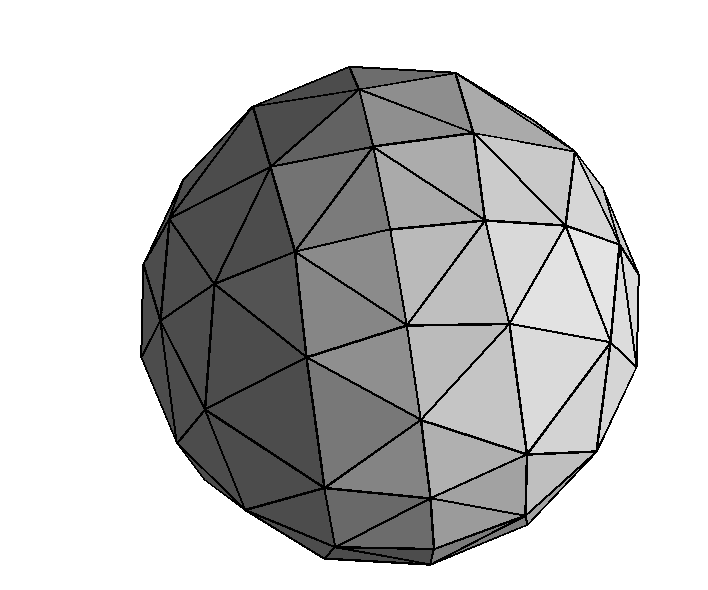
\includegraphics[width=7.5cm]{img/sphere128.pdf}\label{fig:sphere128}}\qquad
	\subfloat[][2048 panels]{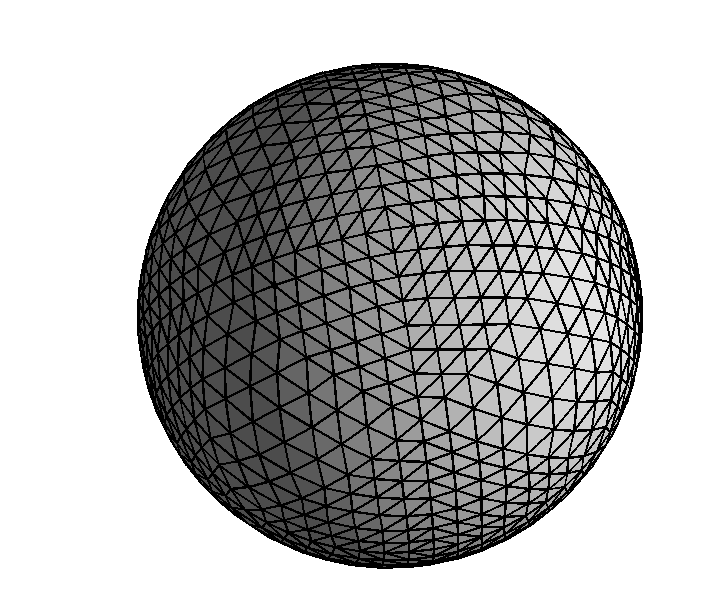
\includegraphics[width=7.5cm]{img/sphere2048.pdf}\label{fig:sphere2048}}\qquad
	\caption{Triangular discretizations of a sphere}
	\label{fig:glob_spheres}
\end{figure}
\end{center}

All tests were performed using a canonical right-preconditioned {\gmres} (algorithm \ref{alg:gmres}) implementation, using our \lstinline|FMM_Plan| framework (see appendix \ref{chapter:fmm_plan}) for the matrix-vector products. We used spherical harmonic expansions for the far-field, and the semi-analytical integral described in \S\ref{subsubsec:semi_analytical} for singular integrals. High precision Gauss quadrature was used for near-singular integrals. In all cases, $\theta_{\text{MAC}} = 0.5$, $p = 10$ and a solver tolerance of $10^{-6}$ was used in order to minimize all but discretization errors.

% Given that the spatial convergence of the collocation method for {\bem} has not been analytically proven, it is important to show that our method behaves as expected. Figures \ref{fig:spatial_convergence_1st} and \ref{fig:spatial_convergence_2nd} show the spatial convergence of the {\fmm}-{\bem} solving  for $\partialdi{\phi}{\hat{n}}$ and $\phi$ respectively. 
%
%\begin{center}
%\begin{figure}[htbp]
%	\subfloat[][1st-kind equation]{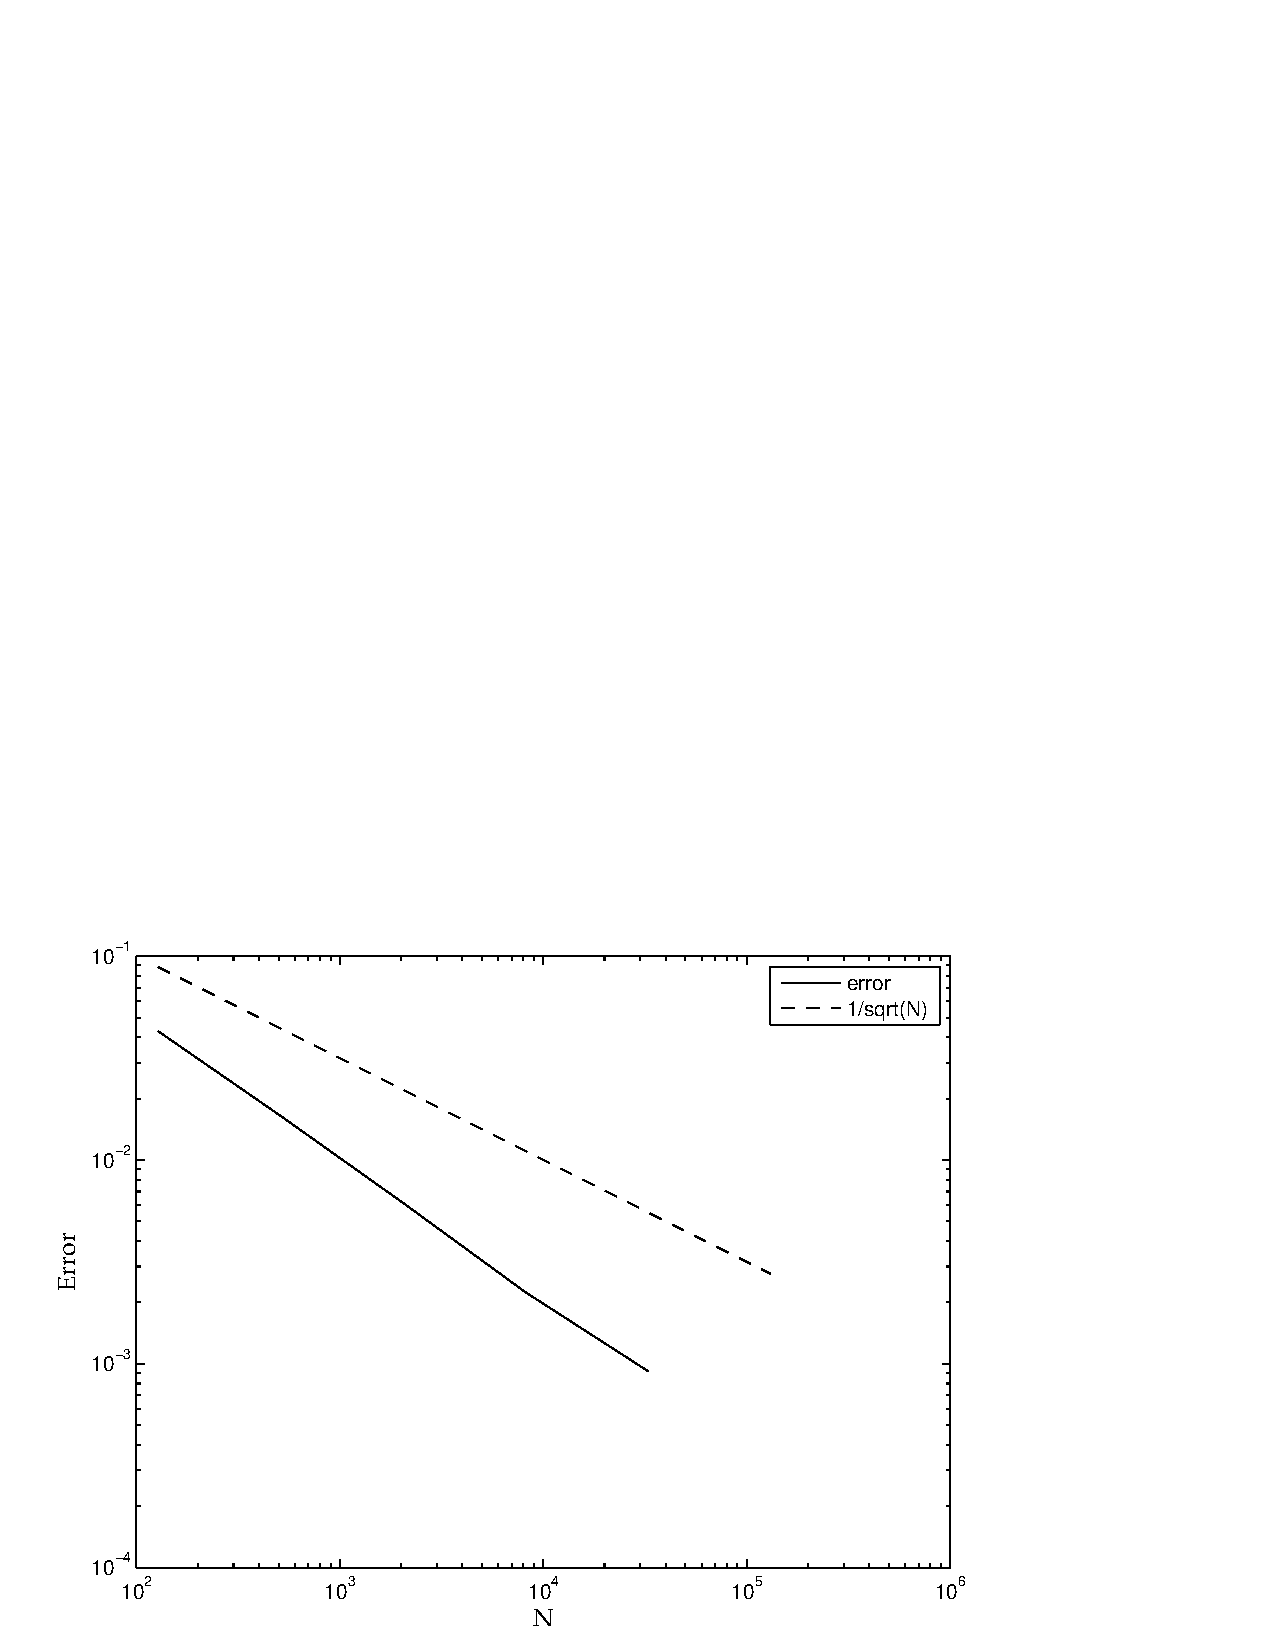
\includegraphics[width=7.5cm]{img/first_kind_convergence.pdf}\label{fig:spatial_convergence_1st}}
%	\subfloat[][2nd-kind equation]{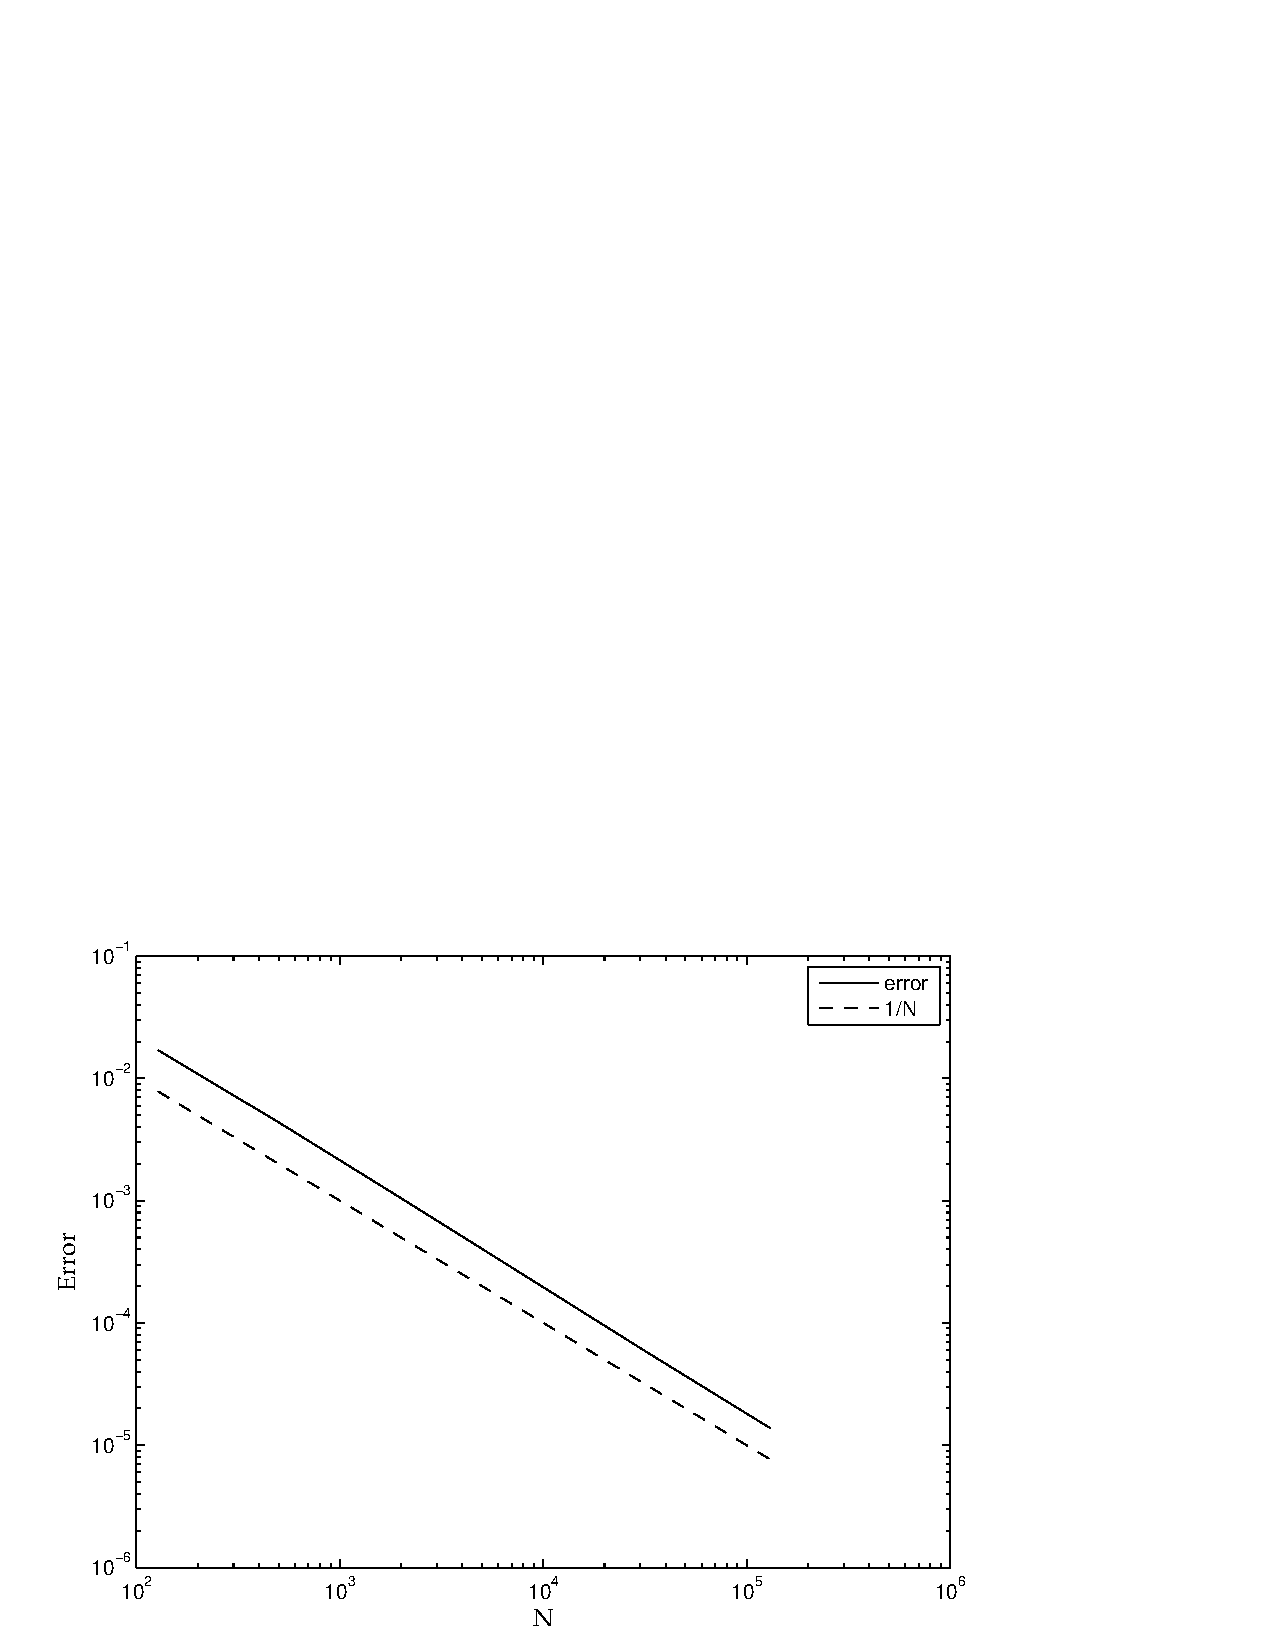
\includegraphics[width=7.5cm]{img/second_kind_convergence.pdf}\label{fig:spatial_convergence_2nd}}
%	\caption{Spatial converge of 1st and 2nd-kind solves}
%	\label{fig:glob_convergence}
%	
%\end{figure}
%\end{center}

\begin{figure}[h]
\begin{center}
	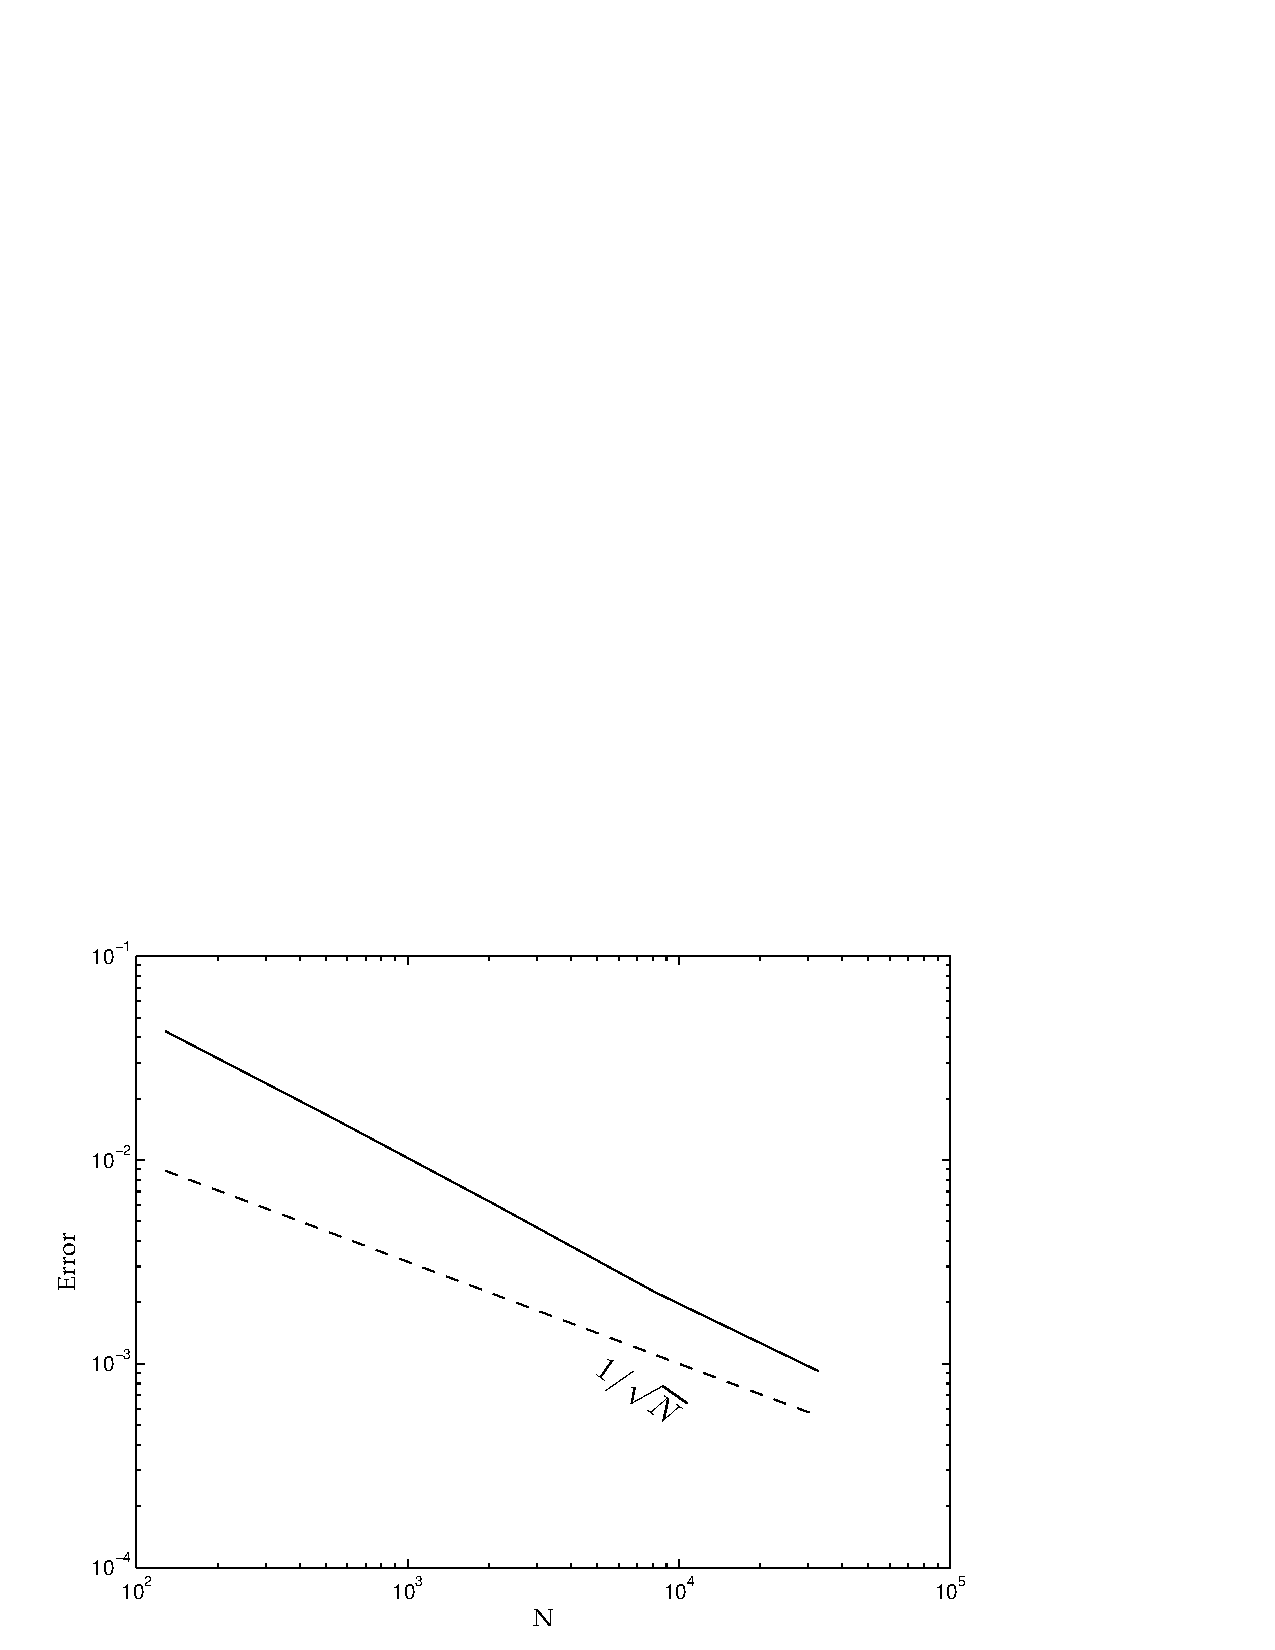
\includegraphics[width=14cm]{img/FirstKindConvergence.pdf}
	\caption{Convergence of 1st-kind solve for Laplace equation on a sphere, solving with $p=10$, solver tolerance of $10^{-6}$.}
	\label{fig:laplace_1st_convergence}
\end{center}
\end{figure}

\begin{figure}[h]
\begin{center}
	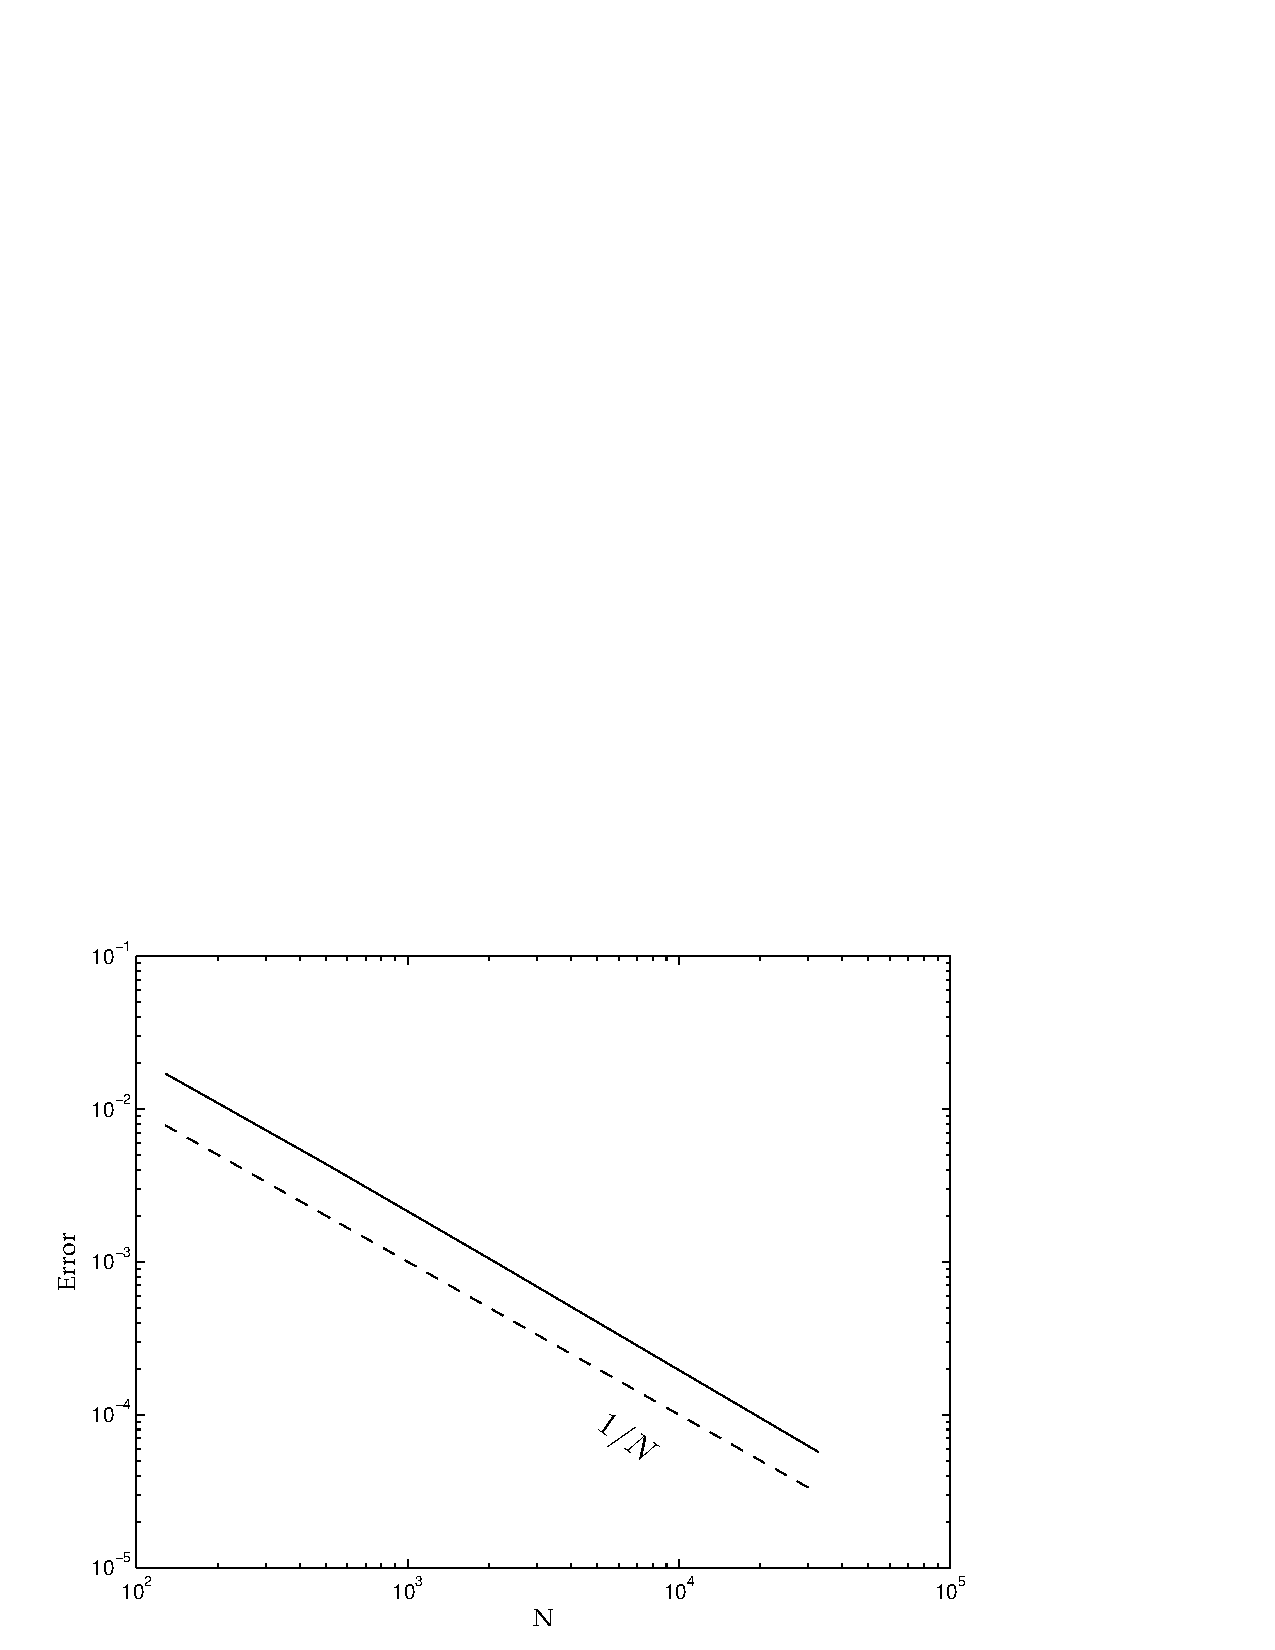
\includegraphics[width=14cm]{img/SecondKindConvergence.pdf}
	\caption{Converge of 2nd-kind solve for Laplace equation on a sphere, solving with $p=10$, solver tolerance of $10^{-6}$.}
	\label{fig:laplace_2nd_convergence}
\end{center}
\end{figure}

Figures \ref{fig:laplace_1st_convergence} and \ref{fig:laplace_2nd_convergence} are encouraging, as they display the correct orders of convergence that we expect compared to comparable codes, namely $\O{1/N}$ for the 2nd-kind solve, while achieving slightly better than $\O{1/\sqrt{N}}$ in the 1st-kind solve. This implies that our {\bem} formulation is correct, the singular / near-singular integrals are accurate, and the far-field approximation using the {\fmm} is also giving the expected answer. This provides the basis we will use to continue experimenting with our code, and ensures that when we use relaxed solvers, we can test their convergence, and be sure that we are still getting the correct answer.

%%%%%%%%%%%%%%%%%%%%%%%%%%%%%%%%%
%%%%% RELAXATION
%%%%%%%%%%%%%%%%%%%%%%%%%%%%%%%%%
\section{Relaxation}\label{sec:laplace_relaxation}

We are trying to minimize the time taken to solve {\bem} problems while not sacrificing accuracy, so it is vital to see how the modifications affect our code's behavior. First, we look at an example problem and see how the residual changes with {\gmres} iterations, and the $p$ required to continue convergence.

\begin{figure}[h]
	\centering
	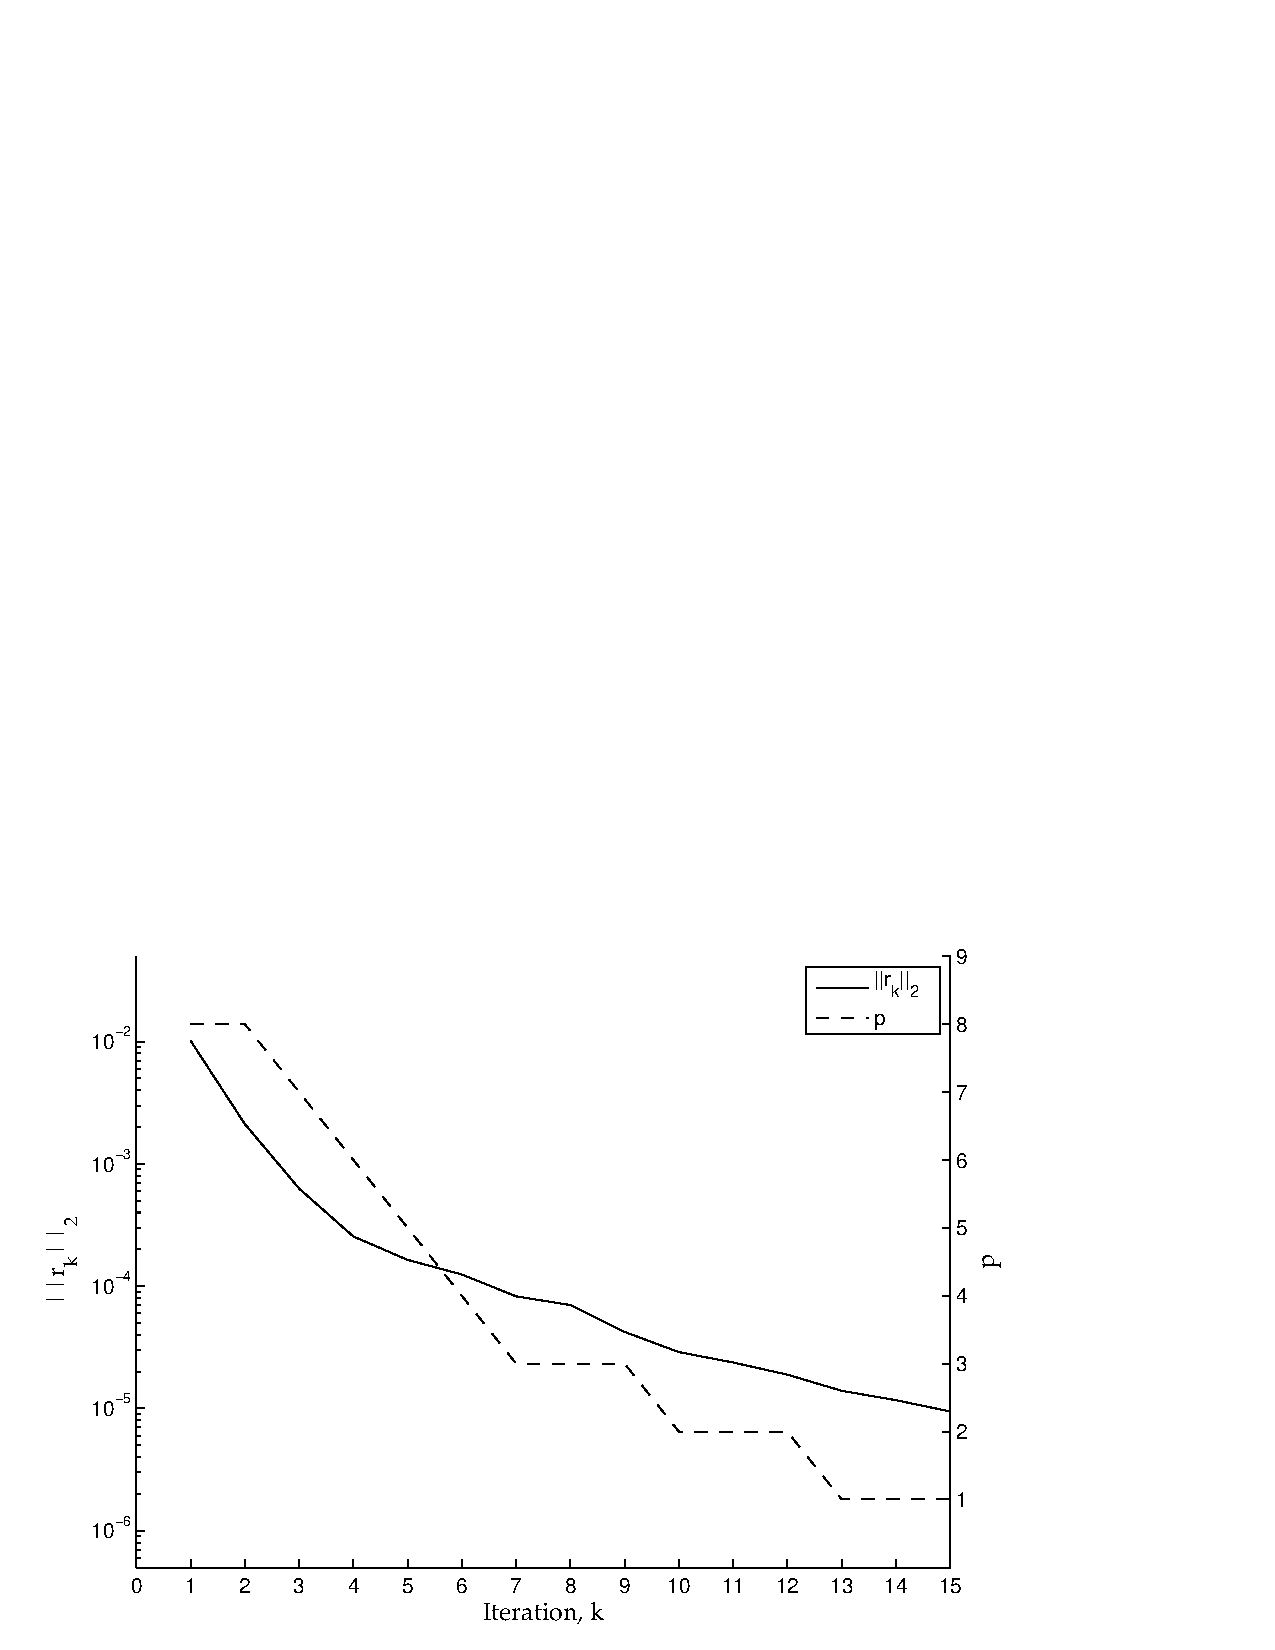
\includegraphics[width=14cm]{img/resid_p_iteration.pdf}
	\caption{Behaviour of the residual $||r_{k}||$ and necessary $p$ against {\gmres} iteration number}
	\label{fig:residualp}
\end{figure}

Figure \ref{fig:residualp} shows how both $||r_{k}||$ and $p$ change over the course of a solve. In this problem, 32768 panels were used to solve the first-kind equation on a sphere to a tolerance of $10^{-5}$ with an initial $p$ set to 8. Clearly, as the residual drops, the $p$ required to maintain convergence of the solver drops significantly, down from $p=8$ at the first iteration to $p=3$ at the 7th. Kernel translation operators in this implementation scale from $\bigO(p^{4})$ for spherical harmonics to $\bigO(p^{6})$ for Cartesian kernels, thus this drop in $p$ can result in large savings in terms of the work being performed. % performance gains.

Next, we compare problems with and without a relaxation strategy. Figure \ref{fig:relaxation_timing} shows the results of tests from 8192 to 131072 panels with a solver tolerance of $10^{-5}$ using a multi-threaded evaluator on 4 cores. For all experiments in this section $\ncrit$ was chosen for each test to minimize the solution time. Only the time spent solving $Ax=b$, $\tsolve$ is plotted. While there are many metrics that could be used to establish performance, we choose to use time-to-solution in all cases for the following reasons:

\begin{enumerate}
\item Reporting times normalized on the number of iterations will both show the same speedups (due to the identical number of iterations required for relaxed and fixed-$p$ solvers), and show exactly the same speedups as the total time-to-solution.

\item Times, rather than operation counts (whether total or per-iteration) are used to abstract away as much as possible the implementation details --- we could potentially use a ``reference operations'' count, the operations required to perform a direct ($\O{N^{2}}$ solve), normalized by either total time (operations per second) or by iterations (average operations per second per iteration), but neither of these options provide any real advantage to simply reporting times.

\item Showing times / operation counts for individual iterations is too unwieldy --- instead of presenting a single value of speedup for each experiment, either multiple values (up to 70+ iterations in some of the later experiments in this thesis) or a plot would need to be presented.
\end{enumerate}

\begin{table}[h]
\begin{center}
\begin{tabular}{c|cc|cc|c}
  & \multicolumn{2}{c|}{Non-Relaxed} & \multicolumn{2}{c|}{Relaxed} & \\
  N & $\ncrit$ & $\tsolve$ & $\ncrit$ & $\tsolve$ & Speedup \\
   & & & & & \\ \hline
   & & & & & \\
  2048 & 400 & 0.27 & 200 & 0.40 & 0.675 \\
   & & & & & \\
  8192 & 400 & 2.58 & 200 & 1.7 & 1.52 \\
   & & & & & \\
  32768  & 400 & 7.1 & 200 & 5.07 & 1.40 \\
   & & & & & \\
  131072  & 400 & 30.1 & 200 & 20.72 & 1.45 \\
 
\end{tabular}
\end{center}
\caption{Speedups for Laplace 1st-kind relaxation, $p=8$, solver tolerance of $10^{-5}$}
\label{tab:laplace_1st_relaxation}
\end{table}%

\begin{table}[h]
\begin{center}
\begin{tabular}{c|cc|cc|c}
  & \multicolumn{2}{c|}{Non-Relaxed} & \multicolumn{2}{c|}{Relaxed} & \\
  N & $\ncrit$ & $\tsolve$ & $\ncrit$ & $\tsolve$ & Speedup \\
   & & & & & \\ \hline
   & & & & & \\
  2048 & 400 & 0.13 & 200 & 0.64 & 0.20 \\
   & & & & & \\
  8192 & 400 & 1.49 & 200 & 1.19 & 1.25 \\
   & & & & & \\
  32768 & 400 & 6.77 & 200 & 5.92 & 1.14 \\
   & & & & & \\
  131072 & 400 & 30.01 & 200 & 24.2 & 1.24 \\
 
\end{tabular}
\end{center}
\caption{Speedups for Laplace 2nd-kind relaxation, $p=8$, solver tolerance of $10^{-5}$}
\label{tab:laplace_2nd_relaxation}
\end{table}%

\begin{figure}[h]
	\centering
	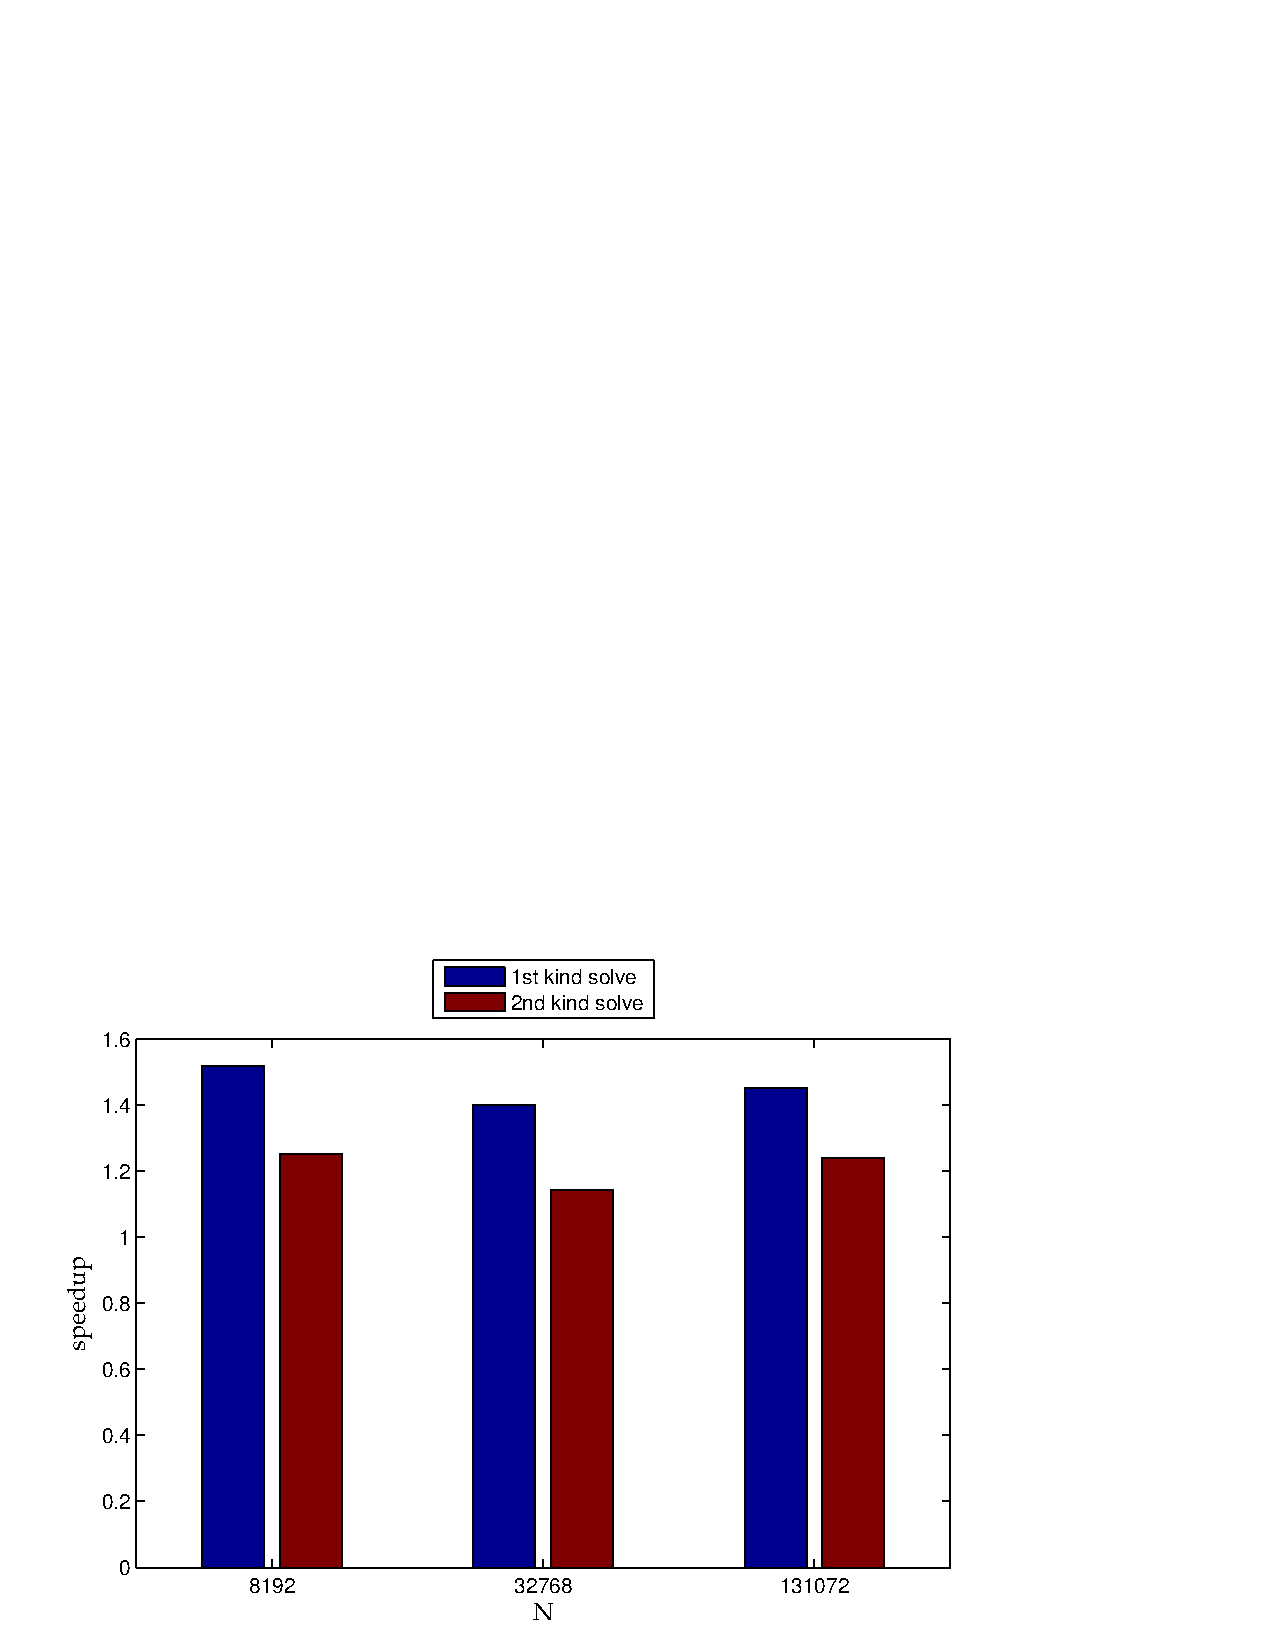
\includegraphics[width=14cm]{img/relaxation_timing_bar.pdf}
	\caption{Speedup using relaxation strategy}
	\label{fig:relaxation_timing}
\end{figure}

From tables \ref{tab:laplace_1st_relaxation} and \ref{tab:laplace_2nd_relaxation}, we can see that there is a benefit from using a relaxation scheme for these problems. For problem sizes of 8192 panels and above, we see an average speedup of around $1.4\times$ for 1st-kind solves and $1.2\times$ for 2nd-kind problems. While these are not huge speedups, they show the first successful application of a relaxation scheme to {\fmmbem}, as well as increasing speedups as problem sizes become larger.

Most interestingly, these results illustrate the differing parameters needed for optimal run times. The best choice of $\ncrit$ changes from $400$ in the non-relaxed case, to $200$ when a relaxed solver is used. This is logical, as for non-relaxed solves the best runtimes will be obtained by balancing the near and far-field evaluations ({\ptop} and {\mtol}). However, when we relax the system, the time taken for the far-field will decrease as a consequence of reducing $p$, while the amount of time for the {\ptop} will remain constant (as an aside, this could also be relaxed, but would necessitate creating a new tree every iteration). This means that to minimize time-to-solution for relaxed cases, we want to reduce this constant {\ptop} cost by adjusting $\ncrit$.

%From this figure, we can see the largest gains, as we might expect, from the larger problem sizes. For these problems, we have deeper trees, and thus more translation operators that will dominate with respect to $p$. This is likely to be the cause of the slightly decreasing speedup for 1st kind equations at the largest tested sizes, as the expensive first iterations dominate the total time taken. The most impressive (and increasing) speedups are for 2nd kind problems, which is encouraging as these constitute many engineering problems (Bioelectrostatics, acoustics).

Now that we have established that relaxation is successful in the sense that it a) converges to the correct answer, and b) provides a speedup in solve times over using a fixed $p$, we can investigate the kinds of situations that will provide the greatest benefits. To do this, we propose 2 hypotheses based on our initial results:

\begin{enumerate}
\item If a higher accuracy (and necessarily higher $p$) is needed, the benefits of relaxation will be greater, due to the ratio of work between the starting and minimum $p$ becoming greater. This hypothesis will be tested by solving a 1st-kind equation for 32768 panels, with varying values of starting $p$. To eliminate potential discrepancies in iteration count between values of $p$, and to recognize that not all problems are as simple to solve as the sphere, we enforce 10 {\gmres} iterations, resulting in a solve to $~5.5\times 10^{-5}$ tolerance. % This is equivalent to solving a slightly harder problem than the sphere, which is known to be comparatively easy. 

\item As more iterations are required, relaxed solves will spend more time at low values of $p$, and thus the speedups will be greater. We will test this hypothesis by artificially increasing the number of iterations in an analogous way to how we fixed the iteration count at 10 earlier. For this particular problem, increasing the number of iterations is equivalent to desiring a lower exit tolerance for the solver. 
\end{enumerate}

We now test both hypotheses, starting with the first; the relation between initial $p$ and overall speedup, using the sphere test case and forcing the solver to perform 10 iterations.

% N vs. p for converged answer
%   2048 : 5
%   8192 : 8
%  32768 : 10
% 131072 : 

% NOTE: at 32768 panels, behaviour is strange -- would need to work with higher k / solver tolerance

\begin{table}[h]
\begin{center}
\begin{tabular}{c|cc|cc|c}
  & \multicolumn{2}{c|}{Relaxed} & \multicolumn{2}{c|}{Non-Relaxed} & \\
  p & $\ncrit$ & $\tsolve$ & $\ncrit$ & $\tsolve$ & Speedup \\
   & & & & & \\ \hline
   & & & & & \\
  5 & 100 & 4.21 & 100 & 6.34 & 1.51 \\
   & & & & & \\
  8 & 100 & 6.24 & 400 & 12.4 & 1.99 \\
   & & & & & \\
  10 & 150 & 8.76 & 400 & 18.5 & 2.11 \\
   & & & & & \\
  12 & 150 & 13.2  & 600 & 25.3 & 1.92 \\
   & & & & & \\
  15 & 150 & 19.3 & 600 & 38.3 & 1.98 \\
 
\end{tabular}
\end{center}
\caption{Laplace 1st-kind relaxation speedup with respect to $p$ for sphere with 32768 panels.}
\label{tab:laplace_1st_p_relaxation}
\end{table}%

\begin{figure}[h]
	\centering
	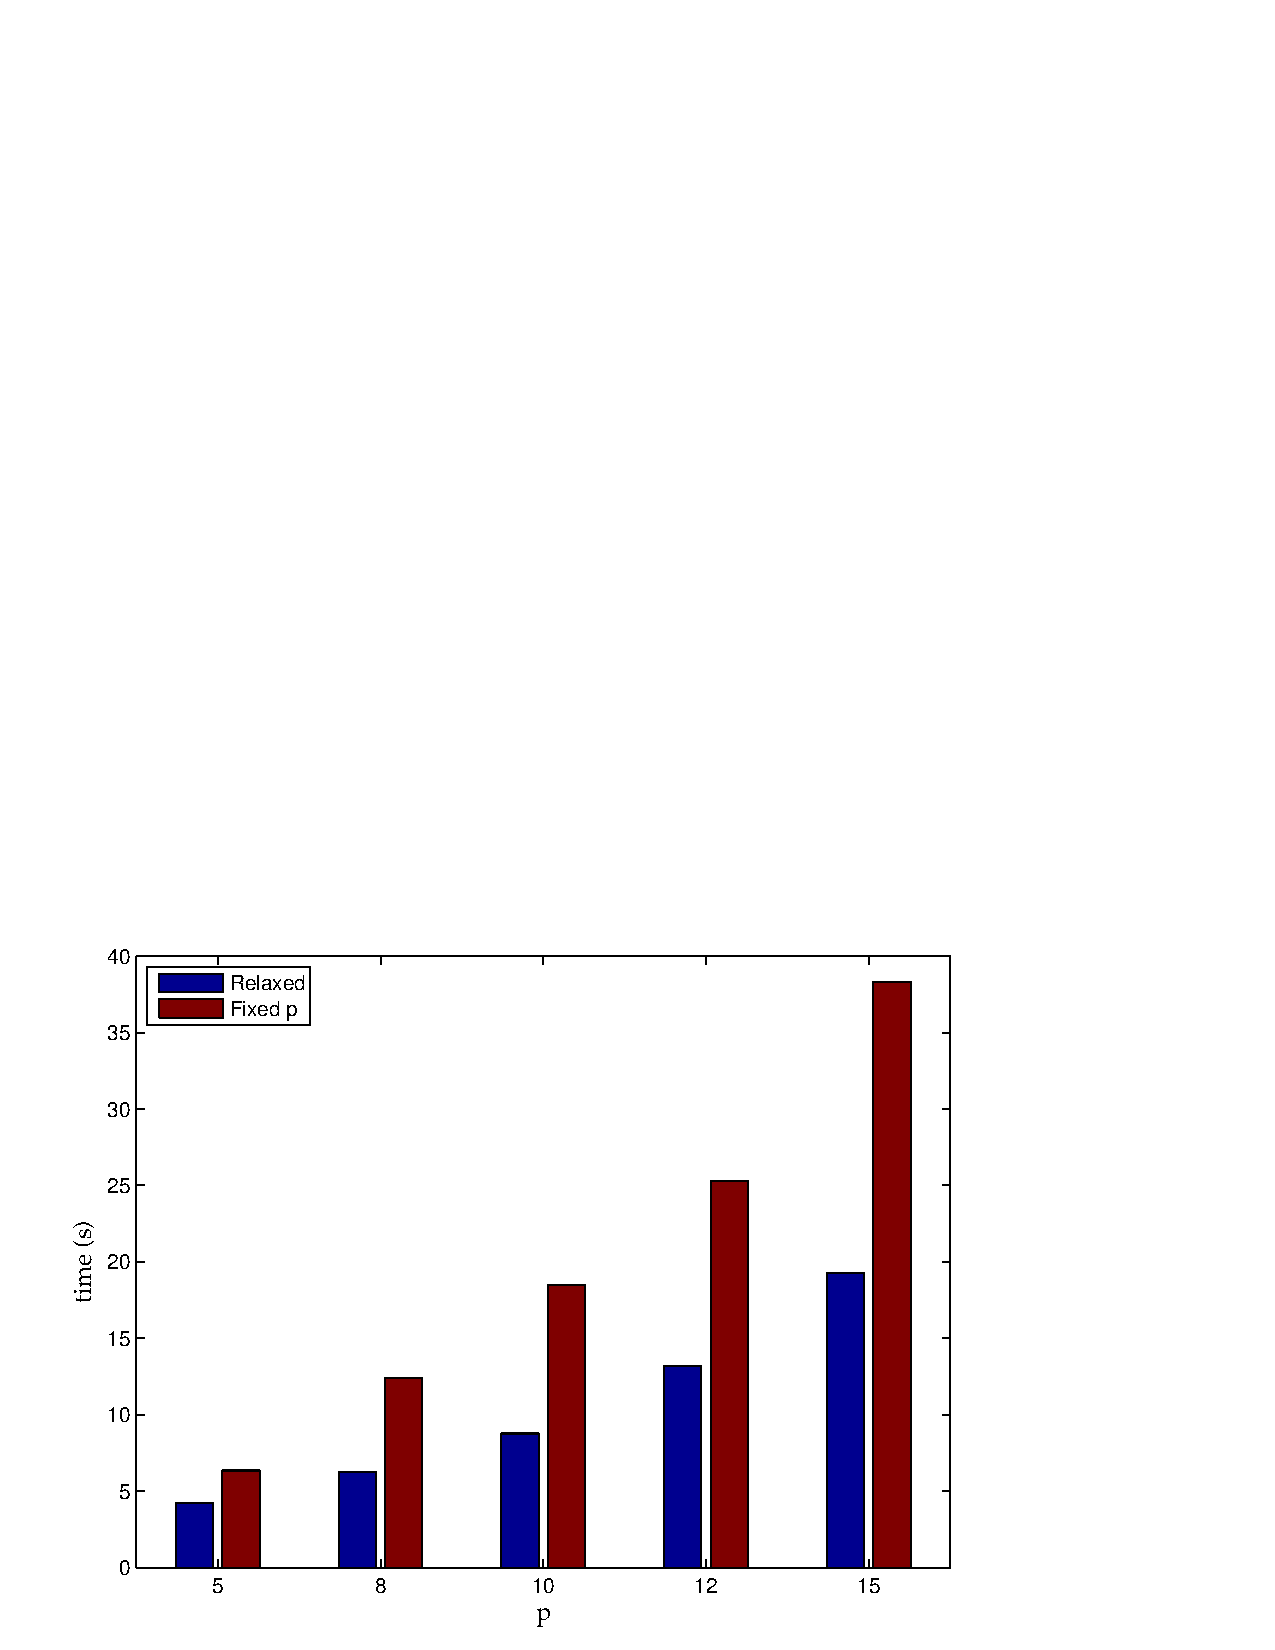
\includegraphics[width=14cm]{img/LaplaceRelaxationP.pdf}
	\caption{Time for 1st-kind Laplace equation solve on a sphere for 32768 panels with varying initial $p$ for relaxed and fixed-$p$ solvers. Iteration count capped at 10 for all cases.}
	\label{fig:laplace_p_speedup}
\end{figure}

The results in table \ref{tab:laplace_1st_p_relaxation} and summarized in figure \ref{fig:laplace_p_speedup} show a general trend -- at the lowest values of $p$ speedup is smaller, but it increases and levels out at approximately $2\times$ for larger tests. Looking at the times taken for individual iterations, this behaviour seems consistent. For the fastest total time, we desire an unbalanced tree on the first iteration (that is, where the time taken for near and far-fields is not equal), with the amount of {\ptop} kept artificially low.

While this means that later, low-$p$ iterations are very quick, it generally results in the first, high-$p$, iterations being slower than the equivalent fixed-$p$ case. Thus, the speedups obtained are purely from the low cost of the last iterations -- with higher $p$, the speedup in these iterations is greater, resulting in lower overall times to solution. The corollary of this, is that for lower initial $p$ the speedups from later iterations is smaller, thus the overall speedup is smaller.

%%% [[[ SPEEDUP TENDING TO NUMBER IF SIMILAR PATTERN OF REDUCING P? ]]]

To test the performance of relaxation with respect to higher iteration counts, we use the sphere problem again, artificially setting the desired number of {\gmres} iterations. This has the effect of progressively solving to lower tolerances, while eliminating potential discrepancies in iteration counts between the relaxed and fixed $p$ experiments. Table \ref{tab:laplace_1st_p_relaxation} shows these results. For all tests, the solver tolerance was disabled and initial $p = 10$. In all cases, a multi-threaded evaluator using 4 cores was used.

\begin{table}[H]
\begin{center}
\begin{tabular}{c|cc|cc|c}
  & \multicolumn{2}{c|}{Relaxed} & \multicolumn{2}{c|}{Non-Relaxed} & \\
  Iterations & $\ncrit$ & $\tsolve$ & $\ncrit$ & $\tsolve$ & Speedup \\
   & & & & & \\ \hline
   & & & & & \\
  5 & 100 & 8.57 & 400 & 10.0 & 1.17 \\
   & & & & &  \\
  10 & 100 & 9.81 & 400 & 18.4 & 1.88 \\
   & & & & & \\
  15 & 100 & 11.1 & 400 & 26.9 & 2.42 \\
   & & & & & \\
  20 & 100 & 12.4 & 400 & 35.3 & 2.85 \\
   & & & & & \\
  25 & 100 & 13.7 & 400 & 43.8 & 3.20 \\
   & & & & & \\
  50 & 100 & 20.6 & 400 & 86.2 & 4.18 \\
 
\end{tabular}
\end{center}
\caption{Laplace 1st-kind relaxation speedup with respect to iteration count for sphere with 32768 panels. $p=10$}
\label{tab:laplace_1st_iterations_relaxation}
\end{table}%

\begin{figure}[h]
	\centering
	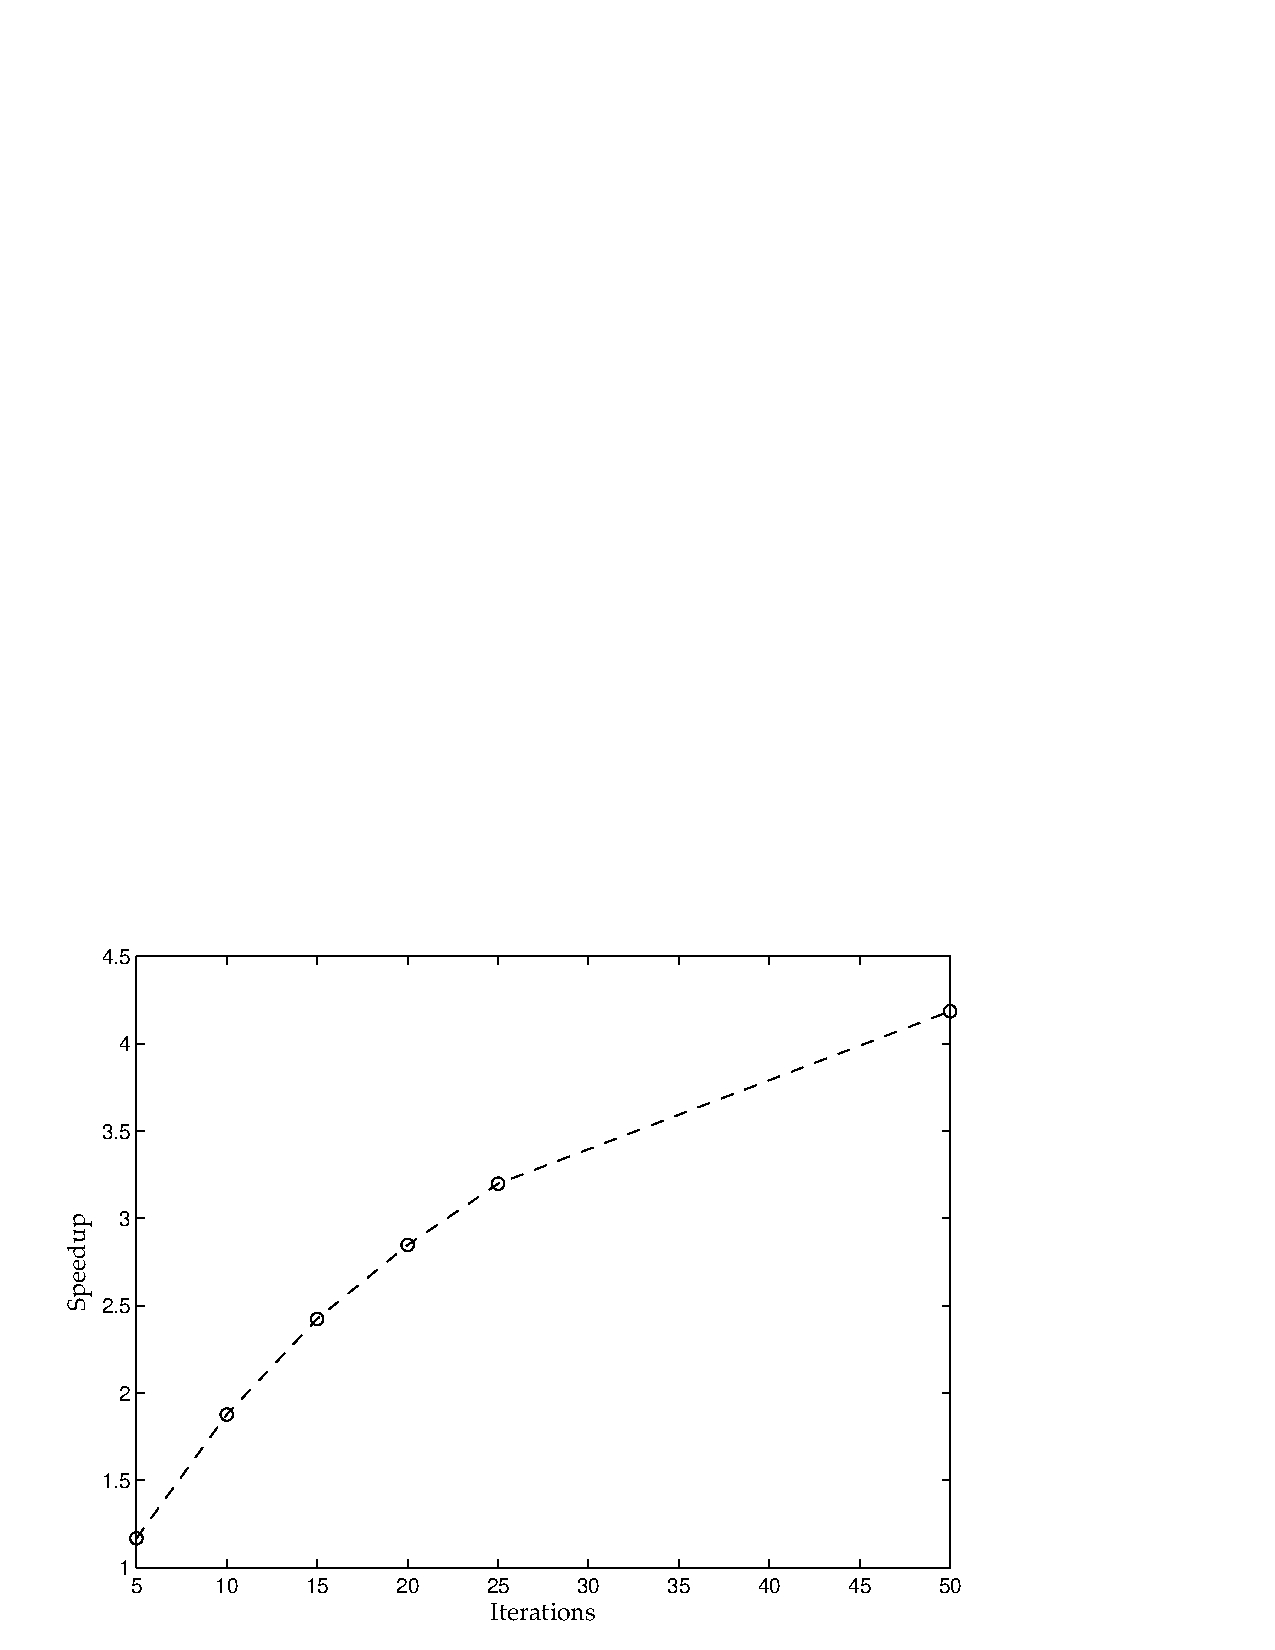
\includegraphics[width=14cm]{img/LaplaceRelaxationIterations.pdf}
	\caption{Speedup of 1st-kind Laplace solve on a sphere for 32768 panels with varying initial iteration count. $p=10$ for all cases.}
	\label{fig:laplace_iterations_speedup}
\end{figure}

From table \ref{tab:laplace_1st_iterations_relaxation} and figure \ref{fig:laplace_iterations_speedup}, the upward trend of speedup with respect to iteration count is very clear. From modest initial speedups, each increase in iterations gives a corresponding increase in acceleration. Further, we can see that each non-relaxed iteration adds approximately $1.68s$ to $\tsolve$, while each relaxed iteration adds a mere $0.276s$. Thus we can predict speedup as the iteration count continues to increase, with a $4.73\times$ acceleration predicted at 75 iterations, and $4.94\times$ at 100 iterations.

Combining our 2 earlier hypotheses and supporting results for both, we can now state that the optimal conditions for speedup from using a relaxation scheme are both a high iteration count, and high desired precision. Any problems exhibiting both these quantities should show significant speedups over standard solvers using a fixed $p$.

\section{Conclusions}\label{sec:laplace_conclusions}

In this section, we have laid the groundwork for applying relaxation schemes to {\fmmbem} problems. We have shown that our implementation is accurate, and that it converges as expected spatially. Beyond that, we have demonstrated the application of a relaxation scheme to {\fmmbem}, the first work of its kind. The parameter space for determining the expected speedup from relaxation has been explored, giving us confidence that any problems that require high accuracy and present tricky linear systems, resulting in many {\gmres} iterations, will give speedups in the order of $2-4\times$, a significant result.

